\chapter{Il sistema analizzato}
\section{Descrizione generale}
Il sistema analizzato rientra nella categoria dei CPSoS. Lo scopo del sistema \`e quello di implementare un meccanismo di posizionamento basato su SFA.\\*
Tale algoritmo viene eseguito da una libreria software schematizzabile, ai fini di questa Tesi, come una \emph{black-box} che rappresenta il nucleo centrale del sottosistema di posizionamento.\\*
Ricevuti in ingresso un certo insieme di misure, essa fornisce in uscita una \emph{stima statistica} della posizione del treno, pi\`u accurata della misura che si otterrebbe utilizzando i dati provenienti dai singoli sensori. \cite{datafuse}\\*
La posizione viene fornita sia in termini di progressiva chilometrica che di coordinate geografiche.
\begin{figure}[h]
	\centering
	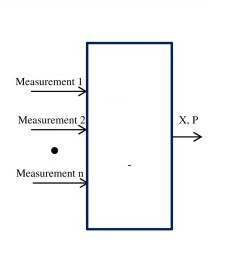
\includegraphics[scale=0.6]{img/sfaschema}
	\caption{Schema SFA}
	\label{fig:sfa}
\end{figure}
\clearpage
SFA viene eseguito su di un hardware installato a bordo treno, e la sua esecuzione \`e volta a monitorare costantemente il moto del treno.\\*
Il ciclo di esecuzione di SFA \`e essenzialmente una continua iterazione di due distinte fasi logiche:
\begin{itemize}
	\item Acquisizione delle misure;
	\item Predizione della posizione del treno.
\end{itemize}
Le grandezze fisiche che dovranno essere misurate e fornite a SFA sono:
\begin{itemize}
	\item Vettore accelerazione;
	\item Vettore velocit\`a angolare;
	\item Coordinate geografiche;
	\item Velocit\`a lineare (scalare).
\end{itemize}
In quest'applicazione, SFA utilizza tali informazioni in combinazione con un'apposita digitalizzazione della traccia tramviaria su cui si trova il treno. \cite{sfaimugps}\cite{sfaimuodo}\cite{sfaimuodogps}\\*
Queste informazioni si suppongono note a priori ed accedibili tramite un \emph{database} caricato in memoria centrale. \cite{sqlite3}\\*
Nel database occorre predisporre una lista di punti geometrici appartenenti alla traccia, caratterizzati dalle loro coordinate e dalla progressiva chilometrica associata. Il sistema modella la traccia come una \emph{spline} interpolante i punti selezionati.
\section{Constituent Systems}
Il sottosistema di posizionamento si compone dei moduli, o CS, descritti nel seguito di questa sezione.
\subsection{Sensor Set}
Il \emph{Sensor Set} \`e un insieme di sensori atti a campionare le misure richieste da SFA. Esso si compone a sua volta dei seguenti moduli:
\begin{itemize}
	\item \emph{Inertial Measurement Unit} (IMU):\\*
		Sensore inerziale incaricato di campionare e trasmettere a SFA i vettori \texttt{accelerazione} ($\mathbf{a}$) e \texttt{velocit\`a angolare} ($\mathbf{v_{ang}}$). Le misure di IMU sono prese rispetto alla Terra e sono espresse in unit\`a stabilite dallo standard internazionale (SI):
		$$
		\mathbf{a}\;\left[\frac{m}{s^2}\right]\;\;\;\;\mathbf{v_{ang}}\;\left[ \frac{rad}{s} \right]
		$$
		IMU \`e il sensore principale su cui si basa SFA nel predire la posizione del treno. Date le caratteristiche intrinseche del particolare SFA utilizzato, ossia un \emph{Filtro di Kalman}, il sistema funziona anche senza i rimanenti sensori. Si osserverebbe tuttavia un calo delle performance in termini di errore commesso sulla stima della posizione del treno. \cite{partialmeas} \cite{gpsdarkarea}
		\begin{figure}[h]
			\centering
			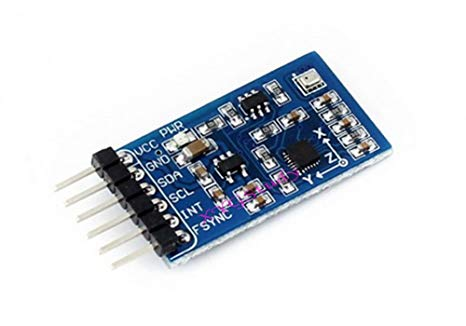
\includegraphics[scale=0.5]{img/imu}
			\caption{\emph{Inertial Measurment Unit}}
			\label{fig:imu}
		\end{figure}
		\item Odometro:\\*
		Unit\`a incaricata di fornire a SFA i valori di velocit\`a lineare del treno, espressi in $\frac{m}{s}$.
		\item GPS:
		\\*Unit\`a che fornisce a SFA le misure di posizione del treno.\\*
Le misure di GPS sono riportate in formato standard come tripla di coordinate \texttt{(latitudine, longitudine, altitudine)}, rispettivamente espresse in gradi \texttt{N-S}, in gradi \texttt{E-O} e in \texttt{metri} sul livello del mare.
\begin{figure}[h]
	\centering
	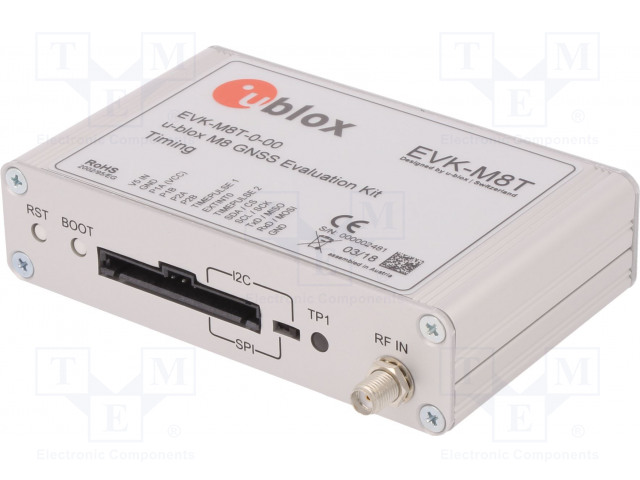
\includegraphics[scale=0.3]{img/gpsublox}
	\caption{Ricevitore \texttt{GPS ublox EVK-M8T}}
	\label{fig:gpsublox}
\end{figure}
\end{itemize}
\subsection{Piattaforma di elaborazione dati}
La piattaforma di elaborazione dati \`e l'hardware sul quale viene eseguito SFA.
Consiste di una scheda \texttt{Nvidia TX-Jetson} collegata al \emph{Sensor Set}.\\*
Da quest'ultimo essa riceve le misure da processare tramite SFA.
\begin{figure}[h]
		\centering
		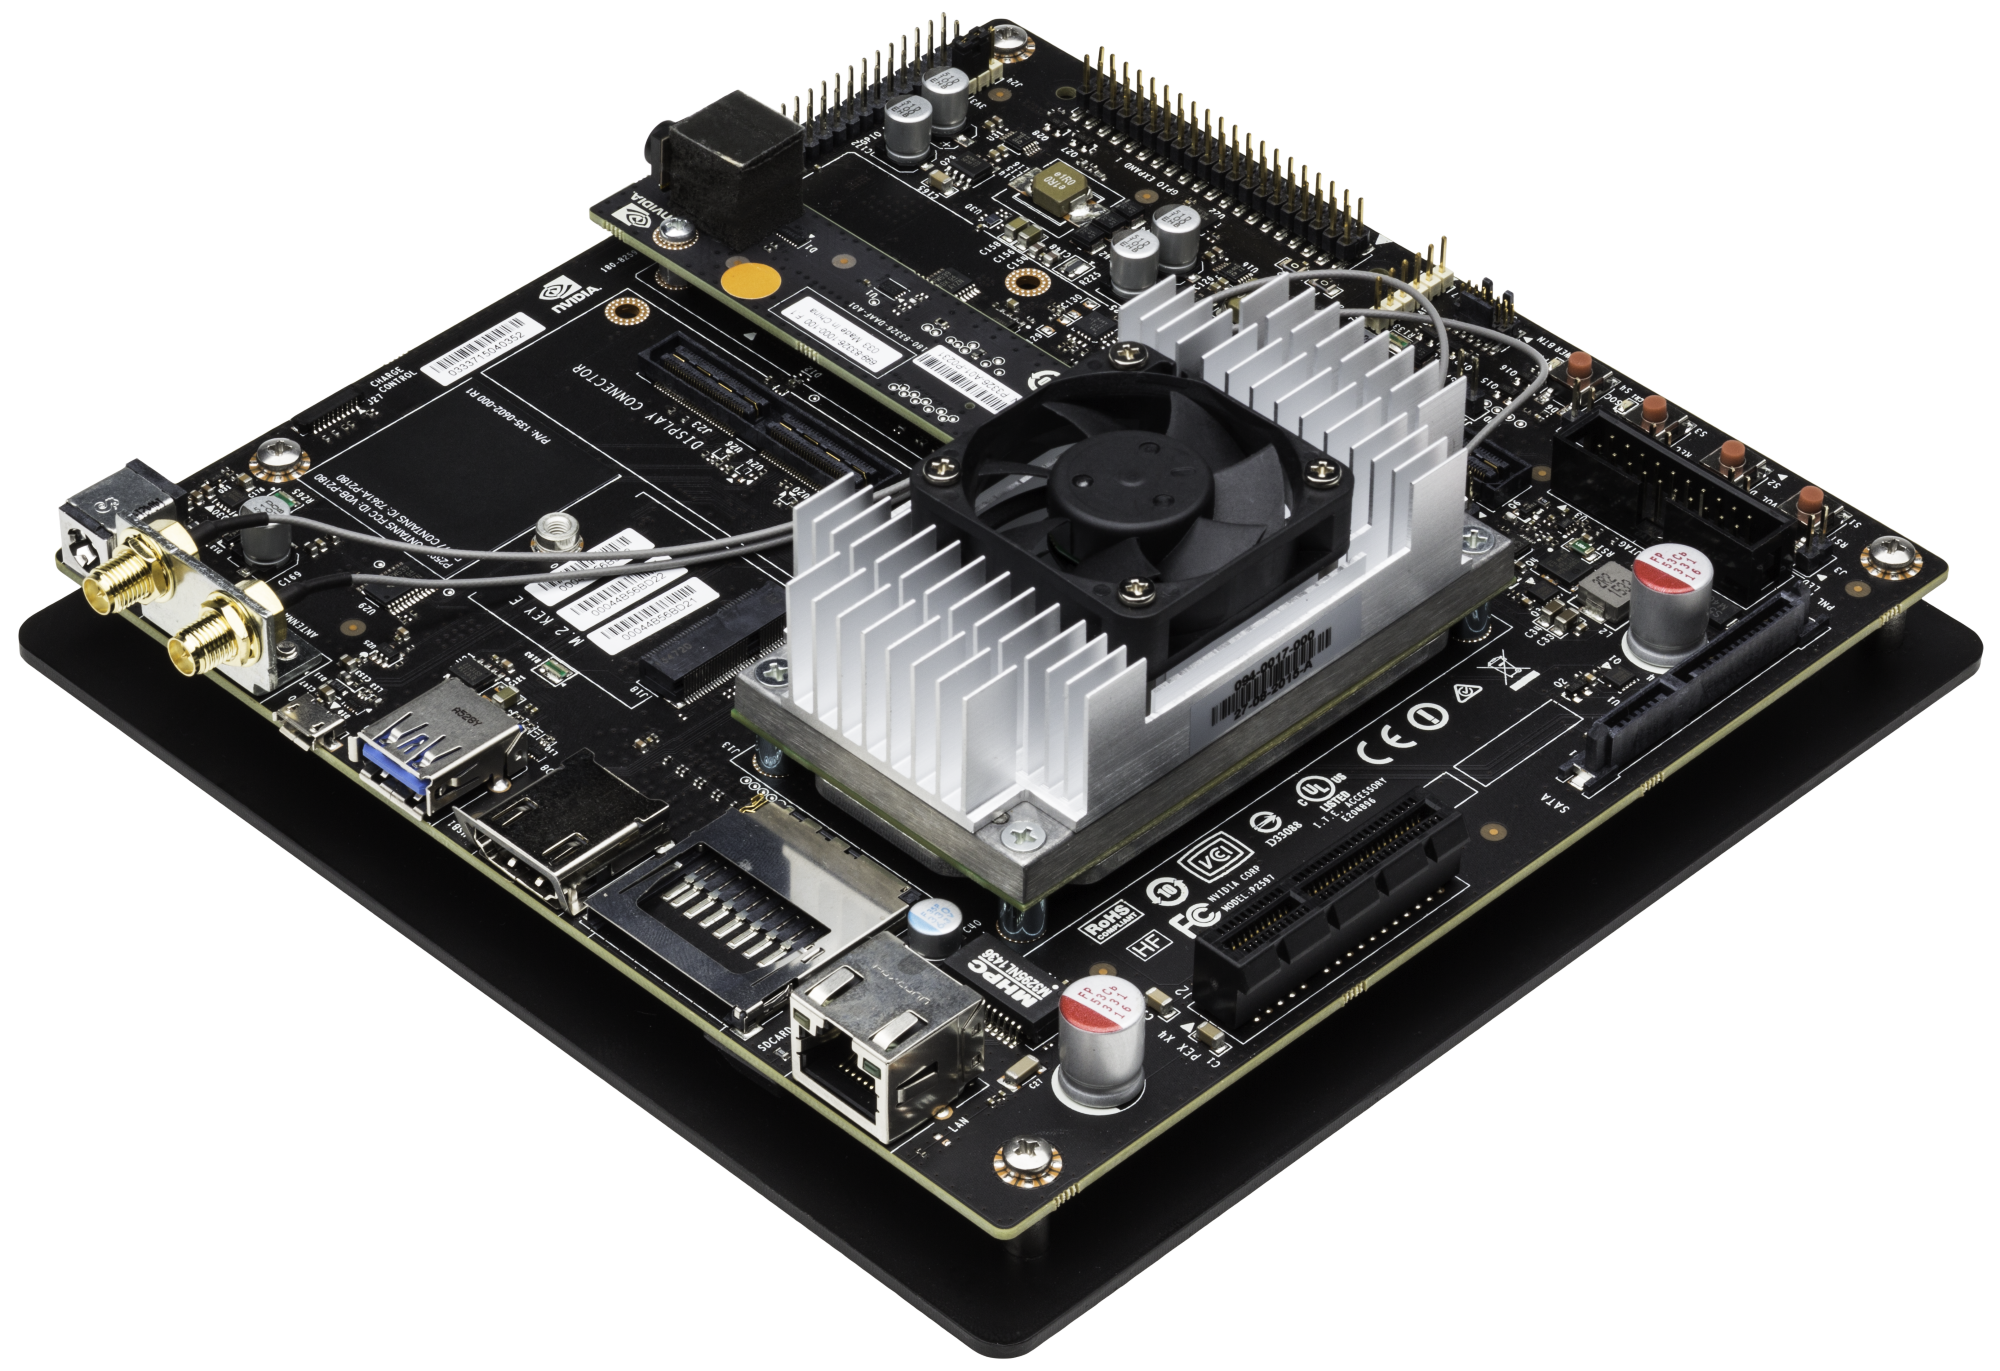
\includegraphics[width=0.7\linewidth]{img/nvidia}
		\caption{\texttt{Nvidia TX-Jetson}}
		\label{fig:nvidia}
\end{figure}
\texttt{Nvidia TX-Jetson} \`e un'architettura specifica per sistemi \emph{embedded}. Essa \`e ottimizzata per i calcoli computazionalmente onerosi tipici delle applicazioni di intelligenza artificiale. \cite{nvidia}\\*
\begin{table}[h]
\begin{tabular}{|p{3cm}|p{8cm}|}
	\hline 
	\textbf{GPU} & 256-core NVIDIA Pascal\\ 
	\hline 
	\textbf{CPU} & Dual-Core NVIDIA Denver 2 64-Bit CPU Quad-Core ARM Cortex-A57 MPCore \\ 
	\hline 
	\textbf{Memoria} & 8GB 128-bit LPDDR4 Memory \\ 
	\hline 
	\textbf{Storage} & 32GB eMMC 5.1 \\ 
	\hline 
	\textbf{Alimentazione} & 7.5W / 15W \\ 
	\hline 
\end{tabular}
\caption{Specifiche Tecniche \texttt{NVidia TX-Jetson}}
\label{tab:nvidia}
\end{table}
\subsection{OBCU}
L'OBCU \`e il computer di bordo del treno. Esso non svolge alcun ruolo attivo nel sistema di posizionamento, tuttavia la progressiva chilometrica, stimata da SFA, dovr\'a essere trasmessa a OBCU al fine di poter utilizzare questa informazione all'interno del sistema di \emph{interlocking} della traccia.
	\section{Specifica delle interfacce}
	\subsection{RUI}
	In questa sezione si evidenziano le principali interfacce del sistema, alle quali si osservano le interazioni fondamentali che avvengono al suo interno.\\*
	Il sistema di posizionamento interagisce con il treno attraverso le RUPI del \emph{Sensor Set}, ossia gli strumenti di misura che esso integra. Questi sensori campionano, a diverse frequenze, i dati sul moto del treno che verranno elaborati da SFA. Una descrizione sintetica delle RUPI del sistema \`e mostrata in tabella \ref{tab:rupi}.\\*
	\begin{table}[h]
	\centering
	\begin{tabular}{|c|c|c|}
		\hline 
		\textbf{RUPI} & \textbf{Grandezza Campionata}  & \textbf{Parti interagenti} \\ 
		\hline 
		Accelerometro & Accelerazione & Vettura - IMU \\ 
		\hline 
		Giroscopio & Velocit\`a angolare & Vettura - IMU  \\ 
		\hline 
		Radar & Velocit\`a lineare & Vettura - Odometro \\ 
		\hline 
		Ricevitore GPS & Coordinate geografiche& Vettura - GPS \\ 
		\hline 
	\end{tabular}
	\caption{Specifica delle RUPI del sistema}
	\label{tab:rupi}
	\end{table}
\FloatBarrier
	Per quanto concerne le RUMI, se ne osservano di due tipi:
	\begin{itemize}
		\item Tre bus dati, che collegano il \emph{Sensor Set} alla scheda \texttt{Nvidia TX-Jetson}. Su ciascuno di essi, \emph{Sensor Set} invia rispettivamente messaggi contenenti i dati campionati da IMU, Odometro e GPS.
		\item Interfaccia LTE. Essa permette di realizzare una \emph{rete wireless ad hoc} fra la scheda e OBCU.\\*
		All'interno di tale rete vengono instradati datagrammi \texttt{UDP} contenenti le informazioni sulla progressiva chilometrica stimata da SFA, ed eventualmente messaggi di \emph{acknowledgment} di OBCU verso la scheda.
		\begin{figure}[h]
			\centering
			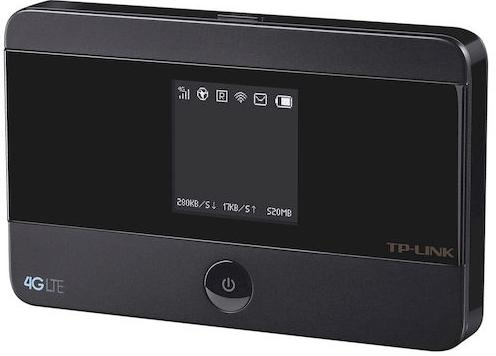
\includegraphics[scale=0.40]{img/lte}
			\caption{Modem \texttt{TP-LINK M7350 LTE-4G}}
			\label{fig:lte}
		\end{figure}
	\end{itemize}
	\begin{figure}[h]
		\centering
		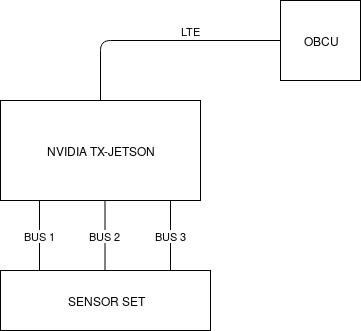
\includegraphics[scale=0.6]{img/TrainDiagram}
		\caption{Diagramma a blocchi del sottosistema di posizionamento}
		\label{fig:tdiagram}
	\end{figure}
		\begin{table}[h]
		\centering
		\begin{tabular}{|c|c|c|}
			\hline 
			\textbf{RUMI} & \textbf{Informazione trasmessa}  & \textbf{Parti interagenti} \\ 
			\hline 
			Bus Dati 1 & Accelerazione, Velocit\`a angolare & Sensor Set - \texttt{NVidia TX-Jetson} \\ 
			\hline 
			Bus Dati 2 & Velocit\`a lineare & Sensor Set - \texttt{NVidia TX-Jetson} \\ 
			\hline 
			Bus Dati 3 & Coordinate geografiche & Sensor Set - \texttt{NVidia TX-Jetson} \\ 
			\hline 
			LTE & Posizione del treno & \texttt{NVidia TX-Jetson} - OBCU \\ 
			\hline 
		\end{tabular}
		\caption{Specifica delle RUMI del sistema}
		\label{tab:rumi}
	\end{table}
\section{Interazioni}
	In questa sezione si descrivono le interazioni osservabili alle interfacce sopra descritte. Queste possono essere in prima istanza categorizzate a discrezione della fase di SFA in cui esse avvengono.\\*
	Si distinguono pertanto le interazioni riguardanti l'acquisizione dei dati in ingresso a SFA, e le interazioni riguardanti l'acquisizione da parte di OBCU della posizione del treno.
	\subsection{Acquisizione dei dati}
	L'acquisizione dei dati si divide in due differenti interazioni: la prima, con la vettura, avviene alle RUPI del \emph{Sensor Set}, mentre la seconda avviene alle RUMI bus dati che collegano il \emph{Sensor Set} alla piattaforma di elaborazione dati.\\*
	I moduli che compongono il \emph{Sensor Set} campionano ad una data frequenza le grandezze fisiche che descrivono il moto del treno. Ciascun campionamento fisico \`e seguito dall'invio dei valori letti alla piattaforma di elaborazione dati. I moduli del \emph{Sensor Set} sono tra di loro indipendenti.\\* 
	In figura \ref{fig:seqdiag} viene riportato un \emph{sequence diagram} rappresentante una possibile sequenza di campionamento e invio dei dati.
	\begin{figure}[h]
		\centering
		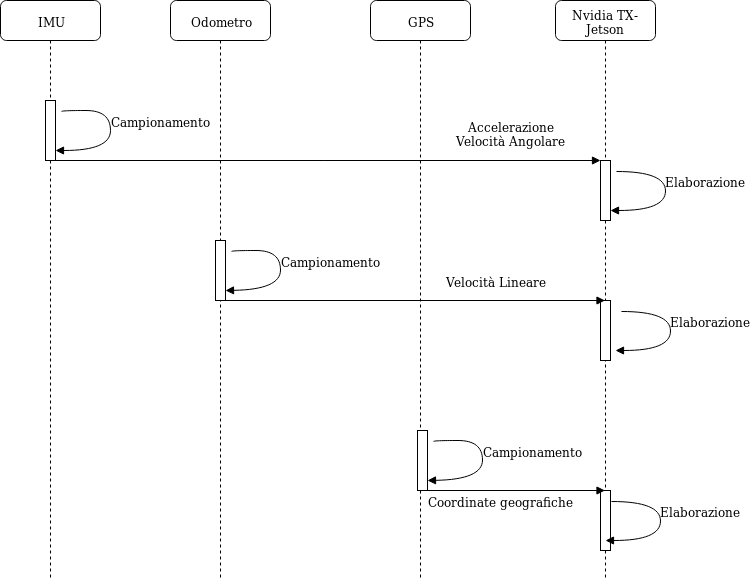
\includegraphics[width=0.7\linewidth]{img/seqdiag}
		\caption{Sequenza di acquisizione dati}
		\label{fig:seqdiag}
	\end{figure}
	Questa tipologia di interazione \`e detta \emph{time-triggered}, in quanto \`e determinata unicamente dallo scorrere del tempo. \cite{timetriggered}
	\subsection{Trasmissione della posizione}
	Ogniqualvolta viene completato un aggiornamento di SFA, si osserva un'interazione all'interfaccia LTE. Tale interazione consiste nell'invio di un messaggio contenente la posizione del treno, dalla piattaforma di elaborazione dati verso OBCU, e nella trasmissione di un messaggio di \emph{acknowledgment} nel senso opposto.\\*
	La tipologia di scambio dei messaggi esposta \`e detta \emph{event-triggered} \cite{evttimetriggered} in quanto le tempistiche di interazione non sono note a priori, ma dipendono dal tempo computazionale impiegato da SFA nell'aggiornare la propria stima della posizione.\\*
	LTE \`e a tutti gli effetti una regolare interfaccia di rete. Il messaggio trasmesso \`e contenuto nel \emph{payload} di un datagramma \texttt{UDP}.
	\begin{figure}[h]
		\centering
		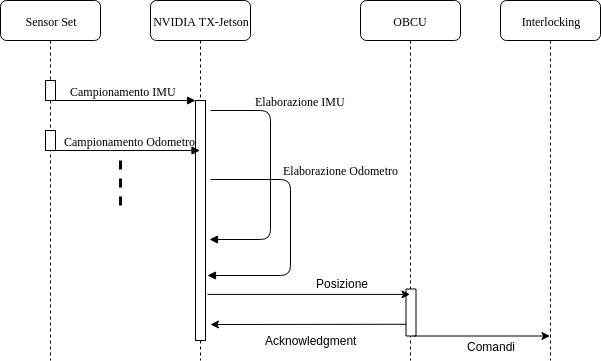
\includegraphics[width=0.7\linewidth]{img/seqdiag2}
		\caption{Sequenza di trasmissione della posizione}
		\label{fig:seqdiag2}
	\end{figure}
	\FloatBarrier
	\subsection{Interazioni con eventuali operatori umani}
	La filosofia del sistema include la minimizzazione di interventi da parte di operatori umani.\\*
	A questi viene lasciato il compito di predisporre le informazioni geografiche della traccia nel database, e di segnalare l'avvio al sistema.\\*
	Il processo che esegue SFA \`e in effetti un \emph{demone} che si avvia contestualmente all'accensione della piattaforma.\\*
	Viene infine predisposta un interfaccia \texttt{SSH} per accedere da remoto alla piattaforma a scopi di \emph{deployment} o di \emph{monitoring online} attraverso la lettura dei file di \emph{log}.
\section{Architettura Software}
In questa sezione viene completata la panoramica sul sistema descrivendo i moduli software in esecuzione sulla piattaforma \texttt{NVidia TX-Jetson}. Su tale piattaforma  \`e installato il sistema operativo \texttt{Ubuntu 16.04 LTS}, basato su Kernel \texttt{Linux}.
\subsection{Sensor Fusion Library}
Il software che esegue SFA viene fornito come libreria, denominata \textit{SensorFusionLib}, la quale mette a disposizione dei \emph{client} le \texttt{API} descritte di seguito.
\subsubsection{API}
Le \texttt{API} di \emph{SensorFusionLib} definiscono le interfacce software verso il modulo SFA che possono essere utilizzate dai \emph{client}.\\*
Le principali funzioni disponibili sono le seguenti:
\begin{itemize}
	\item \texttt{FusionInit(args...)}\\*
	Funzione che inizializza SFA. Tale funzione deve essere chiamata quando \`e necessario avviare l'algoritmo. Essa riceve come parametri i valori che caratterizzano le condizioni iniziali del moto, come l'errore iniziale rispetto alla progressiva chilometrica e alla velocit\`a;
	\item \texttt{ProcessInertialMeasurementData(args...)}\\*
	Funzione che permette a SFA di ricevere ed elaborare un campionamento di IMU; 
	\item \texttt{ProcessOdometryMeasurementData(args...)}\\*
	Funzione che permette a SFA di ricevere ed elaborare un campionamento di Odometro;
	\item \texttt{ProcessGPSMeasurementData(args...)}\\*
	Funzione che permette a SFA di ricevere ed elaborare un campionamento di GPS;
	\item \texttt{ProcessStrobe(args...)}\\*
	Funzione che deve essere invocata ogni secondo, per permettere a SFA di sincronizzarsi rispetto a una \emph{global timebase} esterna; \cite{clock}
	\item 
	\texttt{IsUpdated()}\\*
	Funzione che restituisce \texttt{vero} se SFA ha completato un'iterazione ed \`e pronto a fornire l'output prodotto;
	\item \texttt{GetFusionOutput()}\\*
	Se \texttt{IsUpdated()} restituisce \texttt{vero}, \`e possibile invocare questa funzione per ricevere da SFA l'ultimo output calcolato.
\end{itemize}
\subsection{Listener}
\textit{SensorFusionLib} \`e incapsulato all'interno di un eseguibile, \textit{listener}.\\*
Questo software possiede un'istanza di \textit{SensorFusionLib} con la quale interagisce attraverso le \texttt{API} descritte in 3.1.1. Esso dispone di due \textit{socket} \texttt{UDP}, una utilizzata per ricevere i dati \textit{raw} provenienti dai sensori, l'altra per la comunicazione remota con OBCU.
\begin{figure}[h]
	\centering
	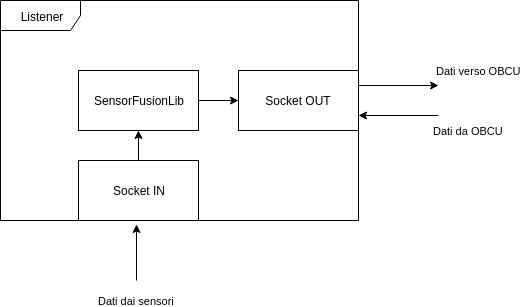
\includegraphics[width=0.7\linewidth]{img/ListenerOK}
	\caption{Diagramma a blocchi di \emph{listener}}
	\label{fig:listener}
\end{figure}
\subsection{Interface Modules}
La comunicazione con i sensori \`e gestita interamente da un set di processi denominati \textit{interface-modules}. Ciascun sensore \`e collegato ad un'interfaccia seriale della piattaforma attraverso un bus dati.
Per ogni interfaccia connessa, un processo resta in ascolto su di essa. Quando un sensore invia un campionamento su una specifica interfaccia, il processo in ascolto su quest'utlima si fa carico di inoltrare a \emph{listener} i valori ricevuti.\\*
Ciascun processo di \emph{interface-modules} dispone di una \emph{socket} \texttt{UDP} che abilita la comunicazione con \emph{listener}.
\begin{table}[h]
	\centering
	\begin{tabular}{|c|c|c|}
		\hline 
		\textbf{Modulo} & \textbf{Sensore}  & \textbf{Dati Inviati a \emph{listener}} \\ 
		\hline 
		\textit{IMU Process} & IMU & Accelerazione, Velocit\`a angolare \\ 
		\hline 
		\textit{ODO Process} & Odometro & Velocit\`a lineare  \\ 
		\hline 
		\textit{GPS Process} & GPS & Coordinate Geografiche \\ 
		\hline 
		\textit{Strobe Process} & N/A & Sincronizzazione \\ 
		\hline 
	\end{tabular}
	\caption{Moduli di \textit{interface-modules}}
	\label{tab:interfacem}
\end{table}
\begin{figure}[h]
	\centering
	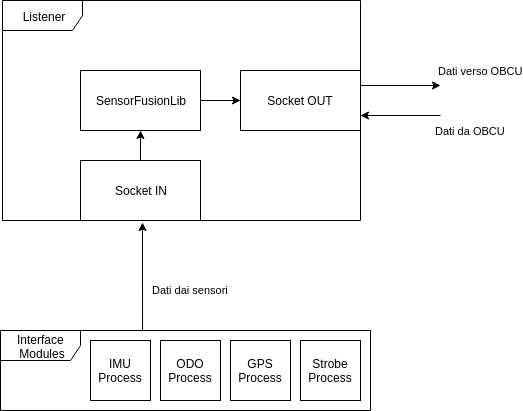
\includegraphics[width=0.7\linewidth]{img/IntModules}
	\caption{Diagramma a blocchi del sistema software}
	\label{fig:imod}
\end{figure}